

\documentclass[a4paper,titlepage]{ctexart}
%\documentclass[a4paper,titlepage,uplatex,dvipdfmx]{jsarticle}

\special{pdf:encrypt ownerpw (1767325) length 128 perm 4}
\linespread{1.5}
\usepackage{siunitx}
\usepackage[version=4]{mhchem}
\usepackage{amsmath}
\usepackage{amssymb}
\usepackage{amsfonts}
\usepackage{metalogo}
\usepackage{appendix}
	\renewcommand{\appendixtocname}{附录}
	\renewcommand{\appendixpagename}{附录}
\usepackage{xcolor}
	\pagecolor[RGB]{46,46,46}
	\color[RGB]{248,248,248}
\usepackage{setspace}
\usepackage{framed}
\usepackage{tabularx}
\usepackage{colortbl}





\usepackage{graphicx}
\usepackage{subfigure} 
\usepackage{float} 
\usepackage{footmisc}

\usepackage[hyperref=true,backend=biber,url=false,doi=true,dateabbrev=true,backref=true,style=numeric-comp,maxnames=15]{biblatex}
\DeclareFieldFormat{biblabeldate}{\mkbibparens{\mkbibbold{#1}}}
\DeclareFieldFormat[article,periodical]{date}{\mkbibbold{#1}}
\DeclareFieldFormat[article,periodical]{volume}{\mkbibbold{#1}}
\DeclareFieldFormat[article,periodical]{number}{\mkbibbold{#1}}
\renewbibmacro{in:}{}
\addbibresource{reference.bib}%导入bib文件。
\usepackage{hyperref}
	\hypersetup{
		bookmarksnumbered=true,
		colorlinks,
		linkcolor=blue,
		urlcolor=blue,
		citecolor=black,
		pdfauthor= {xyx},
		pdfsubject={LaTeX简明手册},
		pdfkeywords={XeLaTeX, upLaTeX, ctex, macro, xeCJK}
	}
	
	
	

\title{README}
\author{xyx}
\date{\today}



\begin{document}

\maketitle
\tableofcontents
\thispagestyle{empty}
\setcounter{page}{0}
\clearpage

\setcounter{section}{-1}
\section{文章整体结构}

\begin{spacing}{1}
	\begin{framed}
		\begin{verbatim}
	~~~~~~~~~~~~~~~~~~~~~~~~~(魔法注释)~~~~~~~~~~~~~~~~~~~~~~~~
	~~~~~~~~~~~~~~~~~~~~~~~~~(特殊命令)~~~~~~~~~~~~~~~~~~~~~~~~	
	\documentclass[全局选项]{文档类} %源代码中的百分号代表此行
	往后都是注释
	~~~~~~~~~~~~~~~~~~~~~~~~~~(导言区)~~~~~~~~~~~~~~~~~~~~~~~~~
	~~~~~~~~~~~~~~~~~~~~~~~~~~(导言区)~~~~~~~~~~~~~~~~~~~~~~~~~
	\begin{document}	%此为文章内容开始之标志
		\maketitle
		\tableofcontents
		\setcounter{page}{0}
		\clearpage
		~~~~~~~~~~~~~~~~~~~~~~~~~~~(正文)~~~~~~~~~~~~~~~~~~~~~~~~~
		~~~~~~~~~~~~~~~~~~~~~~~~~~~(正文)~~~~~~~~~~~~~~~~~~~~~~~~~
		\section{节名}
		~~~~~~~~~~~~~~~~~~~~~~~~~~~(正文)~~~~~~~~~~~~~~~~~~~~~~~~~
		\subsection{小节名}
		~~~~~~~~~~~~~~~~~~~~~~~~~~~(正文)~~~~~~~~~~~~~~~~~~~~~~~~~
		\subsection{小节名}
		~~~~~~~~~~~~~~~~~~~~~~~~~~~(正文)~~~~~~~~~~~~~~~~~~~~~~~~~
		\subsubsection{子小节名}
		~~~~~~~~~~~~~~~~~~~~~~~~~~~(正文)~~~~~~~~~~~~~~~~~~~~~~~~~
		~~~~~~~~~~~~~~~~~~~~~~~~~~~(正文)~~~~~~~~~~~~~~~~~~~~~~~~~
		\clearpage
		\bibliographystyle{unsrt}	%标明参考文献的样式
		\bibliography{reference.bib}	%引入参考文献, 大括号内为文献
		表位置
		
		\clearpage	%新起一页
		\appendixpage	%生成附录页
		\noappendicestocpagenum	%命令目录中的“附录”字样后方不标
		页码
		\addappheadtotoc	%将“附录”字样加入目录中
		\appendix	%规定此后为附录环境
		\section{附录标题}
		~~~~~~~~~~~~~~~~~~~~~~~~~(附录正文)~~~~~~~~~~~~~~~~~~~~~~~
		
		(此后结构可同正文, 但习惯上没有subsection和subsubsection)
		
	\end{document}	%此为文章内容结束之标志
		\end{verbatim}
	\end{framed}
\end{spacing}
此后不再附注源代码, 可以在本地编译之后, 用\href{https://www.texstudio.org/}{TeXstuido}等编辑器的源代码$\longleftrightarrow$ \verb|pdf|双向跳转功能对各个效果进行查看.

\subsection*{魔法注释}
魔法注释的作用一般是指定编译器. 如果用\LaTeX 专用编辑器, 或是编译环境较为固定则是没有什么太大必要学. 但是一些人用Emacs, Vim等编辑器则需要进行设定. 本文未使用魔法注释.
\subsection*{特殊命令}
%特殊命令目前仅需要一个加密命令. 但这个加密命令对复制进行的限制, 目前发现只对网页浏览器等自带的pdf浏览器有效; 若使用\verb|Skim|, \verb|SumatraPDF|等查看则不受限制. 本文仅使用了加密这一条特殊命令. 加密命令的详细使用方法见\href{https://blog.si-on.top/2021/LaTeX-Encrypt/}{此处}
\clearpage

\section{文档类}
\par
\LaTeX , pdf\LaTeX, \XeLaTeX, Lua\LaTeX, up\LaTeX 有对\verb|UTF-8|字符集的支持, 但默认仅显示\verb|ASCII|字符集, 需要额外的调用才会生成\verb|UTF-8|字符集. 其中\XeLaTeX 与Lua\LaTeX 支持从编译者的电脑字体库中调用字体, 而别的均依赖\LaTeX 内的字库. 而中文目前已经几乎完全基于\verb|UTF-8|, 这意味着我们只需要调动相应的字符集就可以让\LaTeX 输出含中文的\verb|.pdf|, 也就是\verb|ctex|宏包. 它需要在导言区被调用. 
\par
\verb|ctex|在不同的编译引擎中会自动选择不同方式实现中文: 它内部包含了不同的宏包, 详见其\href{http://mirrors.ctan.org/language/chinese/ctex/ctex.pdf}{官方文档}. 换言之, 若单独调用其启用中文的核心组件, 也可以实现中文. 但是目录页等字样会保持英文: 对它们的翻译基于\verb|ctex|. 东亚文字的数字化开发一般都是一同进行, 所以也可以通过类似的方法轻量化实现日文, 此处不再赘述.


\par
但是这个\verb|.tex|文件的导言区内并没有调用\verb|ctex|或其他调用中文的宏包, 是因为使用了\verb|ctex|文档类之\verb|ctexart|. 另外还有3种\verb|ctex|文档类: \verb|ctexrep|, \verb|ctexbook|, \verb|ctexbeamer|. 它们分别对应了英语格式的\verb|article|, \verb|report|, \verb|book|, \verb|beamer|并有对全角字符的格式优化. \verb|ctex|文档类现已集成于国际各主流\LaTeX 发行版基础组件中.
\par
文档类文件一般包含在基础组件内. 若要向学术期刊投稿, 需要按照他们模板制作文档, 此时他们会提供\LaTeX 模板文件, 类比定义了\verb|ctexart|的文件. 若在导言区填入了一个非系统自带的, 则这个格式定义文件, \verb|.cls|文件, 须和文档在同一个文件夹内. 一般学术期刊提供的模板不仅仅是\verb|.cls|文件, 是一个还包括了更多的样式定义文件的压缩包, 故而推荐将其解压后直接在其文件夹内部进行文档编辑与编译.

\clearpage

\section{常用功能}
本文采用了适用于大部分化学类文章编写的环境. 从人类认知逻辑上, 我们可以把一个\LaTeX 源代码分为以下几个区域\footnote{大部分我自己取的名, 或者对官方译文有化用}: 

\begin{itemize}
	\begin{spacing}{1}
	\item 导言区:
	\begin{itemize}
		\item 顶级命令区
		\item 样式调用区
		\item 插件调用区
		\item 文章元素规定区
	\end{itemize}
	\item 文章区:
	\begin{itemize}
		\item 正文区
		\item 参考文献区
		\item 附录区.  

	\end{itemize}   
		\end{spacing} 
\end{itemize}

\subsection{特殊命令$\sim$导言区}
\par
各具体设定代码详见源文件. 自上到下各代码分别代表着:
\begin{spacing}{1}
\begin{enumerate}	
	\item 顶级命令区:
	\begin{enumerate}
		\item{加密pdf的特殊命令:} perm后的数字标识了开放的权限, 4为仅允许低质量打印: 点击打印按钮, 如果输出为一个新pdf会发现全部页面都被转化成了低分辨率图片; 2052为仅允许普通打印;此处省略了userpw项, 即打开文档时的密码.
		\item \verb|[|纸张类型+生成标题页\footnote{有则生成, 没有则报错}(+\LaTeX 编译引擎标识+dvi2pdf引擎标识 \footnote{此处仅能提示各组件对其优化,而不是用来指定引擎; 指定引擎另须以魔法注释标明,且须有编辑器支持; 一般仅在使用uplatex+dvipdfmx时须进行此标注,否则会有宏包各种报错})\verb|]|+\verb|{|文档类\verb|}|.
		\begin{itemize}
			\item 中文用\verb|[a4paper,titlepage]{ctex...}|;
			\item 日文用\verb|[a4paper,,titlepage,uplatex,dvipdfmx]{js...}| ;
			\item 详细的通用文档类列表见\href{https://texwiki.texjp.org/?%E3%82%AF%E3%83%A9%E3%82%B9%E3%83%95%E3%82%A1%E3%82%A4%E3%83%AB%E4%B8%80%E8%A6%A7/}{此处}.
		\end{itemize}
	\end{enumerate}
	\item 样式调用区:
	\begin{enumerate}
		\item 定义行距为1.5倍;
		\item 调用物理单位样式的宏包\verb|siunitx|: 在公式环境中, 可以生成标准样式的带单位物理量;
		\item 调用化学(方程)式的宏包\verb|mhchem|: 调用它时强制要求必须标明宏包版本号, 否则报错;
		\item 调用数学公式样式的宏包\verb|amsmath|: 它提供了多种公式样式以及公式对齐样式;
		\item 调用数学符号样式的宏包\verb|amssymb|;
		\item 调用数学字体样式的宏包\verb|amsfonts|;
		\item 调用记号样式的宏包\verb|metalogo|;
		\item 调用附录样式的宏包\verb|appendix|;\label{附录导言区}
		\begin{itemize}
			\item 基于此宏包, 规定目录中出现“附录"字样, 默认值为不出现, 设为出现时则是出现“Appendices".
			\item 基于此宏包, 规定附录第一页左上角出现“附录"字样, 默认值为不出现, 设为出现时则是出现“Appendices".
		\end{itemize}
		\subitem 调用\textcolor{brown}{颜}\textcolor{red}{色}\textcolor{green}{宏}\textcolor{blue}{包}\verb|xcolor|: 但其实\LaTeX 本身也提供一些默认颜色, 但它可以指定RGB色号.
			\subitem 定义全局背景色为\verb|RGB|值为(46, 46, 46)的颜色\footnote{这是我的编辑界面背景色, 不然左边黑边白太扎眼, 文件正式发布前删掉再跑通就行了};
			\subitem 定义全局文字颜色为\verb|RGB|值为(248, 248, 248)的颜色\footnote{底色偏黑, 那我就随便选了一个偏白的颜色当文字颜色}.
		\item 调用行距调整宏包\verb|setspace|: 基于此宏包, 可以部分调整行距;
		\item 调用文本框生成宏包\verb|framed|: 基于此宏包, 可在被选择的文本外围生成文本框;
		\item 调用表格样式宏包\verb|tabularx|
		\item 调用表格背景色包\verb|colortbl|: 基于此宏包, 可表示\verb|Excel|中的背景色
	\end{enumerate}
	
	\item 插件调用区:
	\begin{enumerate}
				
		\item 调用图片插入宏包\verb|graphics|;
		\item 调用子图插入宏包\verb|subfigure|; 
		\item 调用浮动元素宏包\verb|float|: 多数时候没什么用, 原因后述;
		\item 调用脚注样式宏包\verb|footmisc|: 脚注功能基于\LaTeX 本身, 此宏包并非必要;
		\item 调用超链接宏包\verb|hyperref|: 它的作用不只是超链接, 也可以编辑生成的\verb|.pdf|的属性; 它会“污染"一些别的宏包的命令, 故而其最好是作为最后一个调用的宏包,易于覆盖别的宏包的命令; 易知仅需打印的文档完全不需要此宏包;
		\item 对超链接宏包的设置项:
		\begin{enumerate}
			\item 在pdf阅读器识别到的书签里, 为各个书签前加上章节号;
			\item 对超链接文字进行染色;
			\item 规定文内跳转链接为蓝色;
			\item 规定url超链接为蓝色;
			\item 规定文献引用标签为黑色;
			\item 规定\verb|.pdf|属性中的文章作者为xyx;
			\item 规定\verb|.pdf|属性中的文章主题为\LaTeX 简明手册;
			\item 规定\verb|.pdf|属性中的关键词为\XeLaTeX, p\LaTeX, ctex, marco, xeCJK.
		\end{enumerate}
	\end{enumerate}
	\item 文章元素规定区\footnote{此处还可以有institute等其它项,但暂时不需要}
	\begin{enumerate}
		\item 规定文章标题为《\verb|README|》;
		\item 规定文章作者为xyx;
		\item 规定发行日期为\verb|\today|\footnote{此为自动获取今天日期的命令,但是不能像python那样可以print(1+1)得到输出2; 可在正文中使用}.
	\end{enumerate}
\end{enumerate}
\end{spacing}
\,\\\,\par
以上为导言区的大体设定, 除了基于对宏包的设定需要在其对应宏包之后, 而其余导言区代码则\textcolor{red}{无顺序以及缩进需求}.
\clearpage
\subsection{正文区}
\subsubsection{顶级结构, 目录与标题}
\par
在\verb|\begin{document}|后, 即为文章内容的开始, 标题与目录自然也算是文章的内容. 而整个文章(代码)的结束标志则是\verb|\end{document}|
\par
紧随\verb|\begin{document}|, 我们能看到如下的代码:
\begin{spacing}{1}
\begin{verbatim}
	\maketitle
	\tableofcontents
	\setcounter{page}{0}
	\clearpage
\end{verbatim}
\end{spacing}
它们的含义分别是: 
	\begin{enumerate}
		\item 生成标题
			\begin{itemize}
				\item 若在导言区未用\verb|\title{...}|设定标题, 则会报错;
				\item 若未在\hyperref[titlepage]{此处}标明\verb|titlepage|选项, 则仅会在对应位置的顶部生成标题, 故极度推荐使用\verb|titlepage|选项, 你好我好大家好.
			\end{itemize}
		\item 生成目录;
		\item 强行设定此页的页码为\verb|0|;
		\item 此页余下留白, 即之后的内容新起一页.
	\end{enumerate}


\subsubsection{行文操作}
在写作时, 时常需要进行切换自然段, 顶格另起一行, 强行空行等操作. 以下为其对应样式



\begin{itemize}
\item 切换自然段
\subitem 在原生文档类(\verb|article|等)中, 也可以使用\verb|\paragraph{自然段名}|来新起一段. 此文件基于\verb|ctexart|生成, 故无法演示. 两种方式英语文章中可以使用, 但是中文日文则不推荐有自然段名;
\subitem \verb|\paragraph{自然段名}|会拉大和上一段的间距, 哪怕不写自然段名. 如果想特意拉大段间距, 则可以全部使用\verb|\paragraph{}|;
\subitem \verb|\par|没有自然段名, 而且貌似没有哪里人喜欢用自然段名, 故而这个足够;
\subitem 以下为效果实例.
\end{itemize}

\begin{framed}
\par 这是一段
\par 这是另一段
\paragraph{自然段名} 这是新一段
\paragraph{} 没有自然段名
\par 这是又一段
\end{framed}


\begin{itemize}
\item 顶格另起一行
\subitem 以下为效果实例.

\end{itemize}

\begin{framed}
\par 这是一段\\顶格新起一行
\par 这是另一段
\\顶格再新起一行
\\
顶格又新起一行
\end{framed}


\begin{itemize}
\item 插入空行
	\subitem \LaTeX 貌似原则上不允许在没有内容的一行文字下再空一行, 也就是禁制连续空行. 但是在\verb|ctex|文档类下是可以的. 最保险的办法是在新开的一行里加一个\hyperref[spacing]{空白元素}, 然后再空行, 便是符合规则的;
	
	\subitem 以下为效果实例.
\end{itemize}


\begin{framed}
	\par 这是一段\\顶格新起一行
	\\\,\\\,\\
	空两行然后顶格又新起一行
	\par 这是另一段
\end{framed}

\begin{itemize}
	\item 特殊符号
	\subitem 一些特殊符号需要在公式环境内使用. 考虑到在文字间的使用情景, 那么我推荐调用\hyperref[inline]{行内模式}的公式环境, 或者是\hyperref[verb]{抄写环境}
	\subitem 在全局命令中被广泛使用的\%, \{, \}, $\backslash$四种符号可以通过在代码前面加一个$\backslash$来解决($\backslash$需要公式环境).
\end{itemize}

\begin{itemize}
\item 新起一页
	\subitem 类似于插入空行, \LaTeX 不允许直接插入空白页, 但可以在一个页面内插入\hyperref[spacing]{空白元素}, 然后再新起一页;
	\subitem 插入的空白页也会带有页眉页脚装饰. 若想清除(变成纯白页), 则可以使用\verb|\thispagestyle{empty}|命令清除其所在页的所有装饰元素\footnote{页面计数不会停};
	\subitem 强行改变某个页的页码可以用\verb|\setcounter{page}{整数}|. 同理, 它也可以改变一些其他元素的序号(section, figure等). 当然, 此命令也会影响后续的页码自动增加;
	\subitem 以下为效果实例.
\end{itemize}

\clearpage                 %%%%%%%%%%令其新起一页%%%%%%%%%%
\,                         %%%%%%%%%%空白元素%%%%%%%%%%
\thispagestyle{empty}      %%%%%%%%%%规定此页无装饰(style = empty)%%%%%%%%%%
\clearpage 				   %%%%%%%%%%令其新起一页%%%%%%%%%%
\setcounter{page}{666}     %%%%%%%%%%规定此页页码为666%%%%%%%%%%         
\,                         %%%%%%%%%%空白元素%%%%%%%%%%
\clearpage                 %%%%%%%%%%令其新起一页%%%%%%%%%%
\setcounter{page}{10}      %%%%%%%%%%规定此页页码为10%%%%%%%%%%



\subsubsection{插入元素}
以下为一些常用示例. 更加完整的宏包功能与调用代码可在\href{https://ctan.org/}{CTAN}上搜索包名并查看其官方文档.
\begin{itemize}

	
	\item 插入图片:
			\begin{figure}[H]
			\centering\
			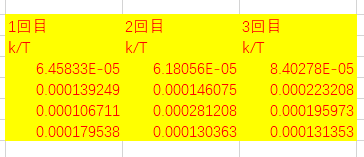
\includegraphics[width=0.5\textwidth]{excel.png}
			\caption{这是题注}
			\label{这是一个文内跳转的地址}
			\end{figure}
						
\begin{itemize}
	\item
此处“图片设定"为\verb|width=0.5\textwidth|, 即一半栏宽; 也可用具体的毫米, 厘米, 英尺等单位: \verb|width=2 cm|; 可指定的数字可以精确到不低于20位小数\footnote{至少20位还没报错, 多了我懒得试, 千分位再往后也没有意义, 因为人看不出来}; 
\item
\verb|[H]|表示作为浮动图形\footnote{没有[T], [B], [P]}强行摆放于此处(Here), 也可使用\verb|[p]|, \verb|[t]|, \verb|[b]|, \verb|[h]|, 它们分别浮动位置的Page of its own(自成一页并摆放在下一页), 表示固定位置的Here(此处), 固定位置的Top(此页顶端), 表示固定位置的Bottom(此页底部). 不标注则摆放位置默认为\verb|[t]|. 也可使用填入多个字母来表示你可接受的摆放方式. 须注意的是, 尽管一般不使用\verb|[p]|, 但它会令此后的内容强制出现在此图片页的后一页: 下一页的正文有且仅有此图片. 若图片以当前设定摆放失败则会自动切换到\verb|[p]|模式;

\item
另有一些其它的图片设定, 例如\verb|angle=30|, 表示图片顺时针旋转$30\unit{\degree}$.此处支持填入大于360的数字;
\item
\LaTeX 支持导入\verb|.png, .pdf, .eps|等格式的图片. 尽管一般可不备注文件后缀名, 但若存在同一文件+多种后缀名的情况, 则会在可导入的文件类型中以拓展名字母顺序(A$\rightarrow$Z)决定导入优先顺序\footnote{不知为何, png的优先级貌似远高于jpg}. 故而此处推荐在代码中标明后缀名, 以避免潜在的报错;
\item 若即将被导入的文件与文档在同一个文件夹内, 则不需额外注明路径; 相应地, 注明路径便能导入电脑里任意位置的图片.

\end{itemize}

\item 子图
	\subitem 效果如下图所示

\begin{figure}[H] 
	\centering
		\subfigure[子图1]{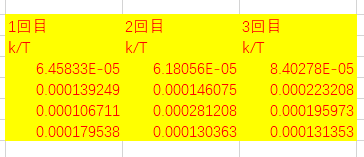
\includegraphics[width=0.48052215576\textwidth]{excel}\label{sf1}}\hspace{0.03\textwidth}
	\subfigure[子图2]{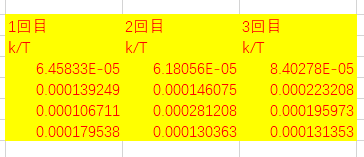
\includegraphics[width=0.48052215576\textwidth]{excel}\label{sf2}}\\
	\subfigure[子图3]{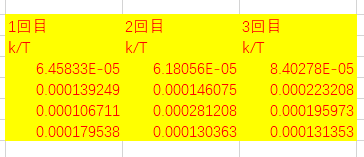
\includegraphics[width=0.48052215577\textwidth]{excel}\label{sf3}}\hspace{0.03\textwidth}
	\subfigure[子图4]{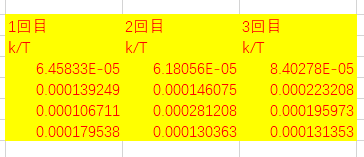
\includegraphics[width=0.48052215577\textwidth]{excel}\label{sf4}}
	\caption{子图示例}
\end{figure}
	\subitem 子图的摆放默认为先横后竖, 且会自动换行, 亦可手动换行. 
	\subitem 注意到:
		\begin{itemize}
			\item \verb|\hfill|命令表示令其前后两元素(即图片)在文字栏内水平等距摆放, 且自动取到最大间距, 亦可在数个元素间加入此命令. 其虽自动, 但是两元素的宽度和超过了\verb|\textwidth|, 则将会失效, 两者将在\verb|\centering|命令下变成页面居中并竖直摆放; 
			\item 亦可用\verb|\hspace{长度}|命令指定两图间距; 
			\item 同一横排的各元素宽度和不应超过0.9910443115\verb|\textwidth|, 否则最右端的元素会被摆放到下一行. 此处指定了每行两图间距均为\verb|0.03\textwidth|; 图\ref{sf1}和图\ref{sf2}宽度均为\verb|0.48052215576\textwidth|, 而图\ref{sf3}和图\ref{sf4}宽度均为\verb|0.48052215577\textwidth|;
			\item 若在两\verb|\subfigure[...]{...}|间插入\verb|\hfill \vrule \\hfill|命令, 则可令两图中央出现一条竖分隔线;
			\item 同理可得: 还有\verb|\vfill|和\verb|\vspace{长度}|命令(V for Vertical, h for Horizontal), 只是一般不用; 亦有\verb|\hrule|.			
		\end{itemize}

\item{公式}\\
 \LaTeX 内自带3种公式环境\footnote{此处是举例环境内, 故而行间公式$\longleftrightarrow$文字间距会很怪, 也受环境影响不会严格居中, 平常不这样}如下:
\begin{itemize}


 \item 行内模式(不支持公式内换行), 其效果为如红色文字所示: \textcolor{red}{$E=mc^2$}\label{inline}
 \item 行间模式(不支持公式内换行), 其效果为如蓝色文字所示: \textcolor{blue}{\[E=mc^2\]}
 \item 带编号的行间模式(不支持公式内换行), 其效果为如绿色文字所示:
 \textcolor{green}{
 \begin{equation}
 	E=mc^2
 \end{equation}}
\end{itemize}

 \subitem 而\verb|amsmath|引入了更多的样式环境如下: 
\begin{enumerate}
	\item \verb|equation*|\footnote{很多时候可用加星号的方式令一个本被计数的环境(section, subsection等)被跳过并不在目录中显示}: 等效于行间模式;\label{电子烟假}
	\item \verb|align|: 可标注行内对齐点的\verb|equation|. 其效果如下灰字所示: 
\textcolor{gray}{
\begin{align}
	1 + 1 & = 2 & & 2 + 2 & = 4 \nonumber \\
1 0 + 1 0 & = 2 0 & & 2 0 + 2 0 & = 4 0
\end{align}}
 它使得不同行的第奇数个\&后的那个字符进行中线对齐, 而第偶数个\&则表示拉开两侧元素的距离; 若不填入任何\&则默认将最长的公式居中, 再令其余向其右对齐.
% \clearpage
	\item \verb|align*|: 不带编号的\verb|align|. \label{spacing}
	\subitem 据前, 易知: 
	
	\begin{itemize}
	\item \textcolor{red}{公式中的字符间距不受源代码的空格影响, 而是自动识别各个字符与命令并摆放}
	\item 若在断行前插入命令可让此行被跳过计数
	\end{itemize}
	\subitem 字符间距自然也可以手动调整, 共有如下6种可选: 
\begin{align*}
1.\,&\Longrightarrow \! \Longleftarrow \text{负空格}\\
2.\,&\Longrightarrow \Longleftarrow \text{无空格}\\
3.\,&\Longrightarrow \, \Longleftarrow \text{窄空格}\\
4.\,&\Longrightarrow \: \Longleftarrow \text{中等空格}\\
5.\,&\Longrightarrow \ \Longleftarrow \text{词间空格}\\
6.\,&\Longrightarrow \quad \Longleftarrow \text{四倍空格}\\
7.\,&\Longrightarrow \qquad \Longleftarrow \text{八倍空格}\\
\end{align*}
\subitem 其中的\verb|\!|, \verb|\,|, \verb|\:|, \verb*|\ |, \verb|\quad|, \verb|\qquad|即为字符间距设置命令.
\subitem 注意到:
\begin{itemize}
\item 此处的\verb*|\ |也被识别为一个命令;
\item 可以用\verb*|\text{ }|命令在公式中插入”文本;
\item 命令间可以紧密相连.
\end{itemize}
\end{enumerate}

	\item 抄写\label{verb}
		\subitem 抄写环境分为行内抄写与行间抄写, 类比与行内公示与行间公式, 此处不再赘述. 每种又分为表示空格与否两种
		\subitem 行内抄写(不表示空格)效果下: \verb|$E=mc^2$ %这是注释|
		\subitem 行内抄写(表示空格)效果如下: \verb*|$E=mc^2$ %这是注释|
		\subitem 行间抄写(不表示空格)效果如下: 
		\begin{verbatim}
			 \begin{equation} %这是注释
				E=mc^2
			 \end{equation} %这是注释
		\end{verbatim}
		\subitem 行间抄写(表示空格)效果如下: 
		\begin{verbatim*}
			\begin{equation} %这是注释
				E=mc^2
			\end{equation} %这是注释
		\end{verbatim*}
		\subitem 注意到:
		\begin{itemize}
			\item 两个|之间的内容将忽略行首行尾缩进的前提下, 忽略区域内一切指令的前提下, 将代码作为文本绝对还原地转写;
			\item 英文与半角符号(\verb|ASCII|字符)转写得到\verb|Courier New|字体, 即老式打印机字体; 
			\item 汉字转写得到\verb|楷体|;
			\item 转写将无法被附加颜色;
			\item 每一个 \verb*| | 符号表示一个半角空格, 而日语中常用的全角空格将会被忽视.
		\end{itemize}
	
	\item 举例
		\subitem 举例环境分为带序号与否2种: \verb|itemize|(不带序号)和\verb|enumerate|(带序号).
		\subitem 两种举例环境可相互混合嵌套: 每一种举例环境最大可以达到4层\footnote{4层itemize加4层enumerate后, 就不能再向其中套任何新的这两种环境了. 实际上只允许套到总计第6层, 但是套到第7和第8也只是报一个非致命错误, 输出文件没问题}, 因为只做了4种不同层级的标识符.
		\subitem 每一个例子还可以分为\verb|item|, \verb|subitem|, \verb|subsubitem|三层, 故逻辑上最高能套到24层. 
		\clearpage
		\subitem 以下为不完全示例:
				
		\begin{itemize}
			\item 第一级
				\subitem 第二级
					\subsubitem 第三级
						\begin{enumerate}
							\item 第四级
								\subitem 第五级
									\subsubitem 第六级
										\begin{enumerate}
											\item 第七级
												\subitem 第八级
													\subsubitem 第九级
											
										\end{enumerate}
						\end{enumerate}	
		\end{itemize}
		\subitem 注意到: 
		\subsubitem 不可在没有\verb|\item|的地方使用\verb|\subitem|; 同理对\verb|\subsubitem|成立;
		\subsubitem 仅\verb|item|前有标识符;, 
		\subsubitem 在\LaTeX 内部的缩进处理中, 无法做到视觉效果的24层, 故而在重复嵌套举例环境中不推荐使用严格的\verb|item|, \verb|subitem|, \verb|subsubitem|.


\item 化学(反应)式
	\subitem 输出效果如下:
	\[\ce{_27Co + 2_26^56Fe ->[\Delta][H2O] Coffee
		->[Human][36\unit{\degreeCelsius}] Pee ->[lake][rt]
		steam (^) ->[sky][winter] {($\pm$)-}$cis/trans$
		{-}snow (v)}
		\]

	\subitem 注意到:
	
	\begin{itemize}
	\item 化学(反应)式可以出现在公式环境内, 也可以出现在正文中, 因为它被别的包调用;
	\item 输入化学(反应)式代码时, 很多命令都跟空格有较强的联系, 故须格外关注; 
	\item 输入化学(反应)式代码时, 在本该有空格的地方选择断行代码则可以不输入空格, 因为断行自带切断作用; 相应地, 乱断行也会造成不必要的麻烦.
	\end{itemize}
	
	
	\item 表格
		\subitem 基于\verb|Excel|的\href{https://ctan.org/pkg/excel2latex}{宏包}\footnote{估计是不支持WPS, 但是正经笔记本都应该是自带了永久Office套装}, 可以将\verb|Excel|的表格导入至\LaTeX. 安装完之后点击顶端``\verb|加载项|''按钮即可看到. 选定想要的区域然后点击\textcolor{red}{不带闪电标}的按钮即可读取此区域的\verb|Excel|布局元素\footnote{Excel的框内文字左/右对齐, 外框线, 合并单元格, 各处颜色等}与内容, 并生成代码. 就目前来看, 如果是把代码粘贴到主文件里, 则必然会无尽报错, 但是如果用\verb|\input{文件名}|命令, 则丝般顺滑:\\ 将生成的表格源代码粘贴进一个空白的\verb|.tex|文件内, 然后放到主文件的同一个文件夹内, 再用
		\begin{spacing}{1}
		\begin{verbatim}
			\begin{centering}
				\input{文件}
			\end{centering}
		\end{verbatim}
		\end{spacing}
		命令即可成功导入如图\ref{这是一个文内跳转的地址}所示的表格. 
		\subitem 带闪电标的按钮说是将所有暂存的源代码输出到\LaTeX, 但实际上这玩意是针对\verb|Offcie2010|开发的, 目前仅能输出选定区域;
		\subitem 被\verb|\input|的文件若标注路径则可实现从电脑的任意处导入代码; 相应地, 若被导入的文件和文档在同一文件夹下, 则不需注明路径.
\begin{centering}	
	% Table generated by Excel2LaTeX from sheet 'Sheet1'
\begin{table}[htbp]

	\centering
	\caption{带背景颜色与文字颜色的表格示例}
	\begin{tabular}{rrr}
		\rowcolor[rgb]{ 1,  1,  0} \multicolumn{1}{l}{\textcolor[rgb]{ 1,  0,  0}{1回目}} & \multicolumn{1}{l}{\textcolor[rgb]{ 1,  0,  0}{2回目}} & \multicolumn{1}{l}{\textcolor[rgb]{ 1,  0,  0}{3回目}} \\
		\rowcolor[rgb]{ 1,  1,  0} \multicolumn{1}{l}{\textcolor[rgb]{ 1,  0,  0}{k/T}} & \multicolumn{1}{l}{\textcolor[rgb]{ 1,  0,  0}{k/T}} & \multicolumn{1}{l}{\textcolor[rgb]{ 1,  0,  0}{k/T}} \\
		\rowcolor[rgb]{ 1,  1,  0} \textcolor[rgb]{ 1,  0,  0}{6.45833E-05} & \textcolor[rgb]{ 1,  0,  0}{6.18056E-05} & \textcolor[rgb]{ 1,  0,  0}{8.40278E-05} \\
		\rowcolor[rgb]{ 1,  1,  0} \textcolor[rgb]{ 1,  0,  0}{0.000139249} & \textcolor[rgb]{ 1,  0,  0}{0.000146075} & \textcolor[rgb]{ 1,  0,  0}{0.000223208} \\
		\rowcolor[rgb]{ 1,  1,  0} \textcolor[rgb]{ 1,  0,  0}{0.000106711} & \textcolor[rgb]{ 1,  0,  0}{0.000281208} & \textcolor[rgb]{ 1,  0,  0}{0.000195973} \\
		\rowcolor[rgb]{ 1,  1,  0} \textcolor[rgb]{ 1,  0,  0}{0.000179538} & \textcolor[rgb]{ 1,  0,  0}{0.000130363} & \textcolor[rgb]{ 1,  0,  0}{0.000131353} \\	
	\end{tabular}%
	\label{RELX5}
\end{table}%

\end{centering}


\item 超链接
	\subitem 常用超链接主要分为以下四种: 
	\begin{enumerate}
		\item 文内指定位置跳转
		\item 获取文内元素代号的跳转
		\item 普通\verb|url|跳转
		\item 带文字的\verb|url|跳转
	\end{enumerate}
	\subitem 超链接跳转基于\verb|hyperref|宏包, 这个宏包的功能包括但不限于生成超链接, 甚至可以更改纸张尺寸和更改\verb|.pdf|文件的属性, 是一个极其强大但混乱的宏包: 它重新定义了许多默认的指令, 生成需要复杂排版的纸质文件时极其推荐不要调用它.
	\subitem 效果如下:
	\begin{enumerate}
		\item 跳转至\hyperref[电子烟假]{这里}
		\item 跳转至\ref{电子烟假} \label{尼古丁真}
		\item \url{https://www.google.com}
		\item \href{https://www.google.com}{PornHub}
	\end{enumerate}
	\subitem 注意到: 
	\begin{itemize}
	\item \verb|\hyperref[落点名]{呈现的元素}|命令中的\verb|呈现的元素|可以是整整一章, 也可以是一整张图, 也可以是一张子图, 也可以是表(具体效果详见附录);
	\item 需要用\verb|\label{名字}|命令来标识超链接的落点位置;
	\item 点击文内跳转超链接后, 落点会在当前显示区域最上方;
	\item \verb|\ref{名字}|命令仅可获取目标的序号, 而不能获取其元素类型(section, figure等), 需要自行注明, 可以参看\hyperref[尼古丁真]{此处}源代码;
	\item 对于图片和表格等元素, 若要作为落点, 则 \verb|\label{名字}|须紧贴相当于\verb|\end{...}|的命令前才可被\verb|\ref{名字}|命令正常识别出其序号, 可见图\ref{sf1}和表\ref{RELX5}的源代码;
	\item {\Huge 慎点超链接, 作者都可能不知道它会跳到哪里}
	\end{itemize}
\clearpage

\item  附录
	\subitem 附录的设置同时需要在\hyperref[附录导言区]{导言区}和附录的代码部分前进行命令.
	\subitem 附录代码处需要用以下命令环绕
	\begin{spacing}{1}
	\begin{verbatim}
		\begin{appendices}
			设定
			\section{...}
			...
			\section{...}
			...
		\end{appendices}
	\end{verbatim}\end{spacing}
	\subitem 此处的\verb|设定|为:
	\begin{verbatim}
\def\thesection{附录\Alph{section}}     
\appendixpage    
\noappendicestocpagenum     
\addappheadtotoc    
	\end{verbatim}

	\subitem 其作用分别为:
		\begin{enumerate}	
		\item 令附录章节名样式变为“附录 A”, “附录 B”\dots;
		\item 令附录第一页的左上角出现标识字样, 字样设定则是在导言区;
		\item 上一条命令定义的标识字样其实也被算作一种有序章节, 故而会在目录中出现页号, 此命令会抹去其页号;
		\item 令“附录”字样出现在目录中.
		\end{enumerate}
	\subitem 易知: \verb|\def\thesection{附录\Alph{section}}|可用于自定义各种元素的序号样式: \label{def}
		\begin{itemize}
			\item \verb|\thesection|中的\verb|section|可以换成\verb|figure|或是\verb|table|等元素名; 
			\item 后面的大括号即为样式设定:
				\subitem 假如我在这里写
				\begin{verbatim}
					\def\thesection{\textit{电子烟假尼古丁真}\alph{section}}
				\end{verbatim}\label{附录文字}
				则之后的附录章节名会变成``\textit{电子烟假尼古丁真} a'', ``\textit{电子烟假尼古丁真} b'', \dots
				\subitem 各部分具体含义如下:
				\begin{enumerate}
					\item \verb|\def|表示对此后的元素重新定义;
					\item \verb|\thesection|表示章节序号样式;
					\item 大括号内即为指定的样式:
						\begin{itemize}
							\item 在\verb|ctex|系列下, 系统会自动在\verb|ASCII|字符和全角字符(汉字)间加入一个半角空格;
							\subitem 相应地, 作为处理中文的格式, 汉字( Chinese characters)间没有空格, 故而在源代码汉字间的空格与断行与不会被识别, 需要用\verb*|\ |命令强加进去;
							\subitem 由于字母语言的特性, 需要用半角空格断字, 若在源代码文字部分的字母间连续输入不少于1个的半角空格或者是断行, 最终也仅会输出一个半角空格;
							\item 可以对此处的内容用命令进行添加下划线, 改变颜色或是变为斜体等操作;
							\item \verb|\alph|表示小写英文字母用作序号, 类似地, 还有: 
							\subitem \verb|\arabic|表示阿拉伯数字;
							\subitem 附录默认的\verb|\Alph|表示大写英文字母;
							\subitem \verb|\Roman|表示大写罗马数字;
							\subitem \verb|\roman|表示小写罗马数字.
							\subsubitem 仅有阿拉伯数字序号可以表示第负数个元素, 其余均不支持非正数序号, 但仅有大/小写英文字母会严重报错, 罗马数字仅会消失;
							\subsubitem  当且仅当序号始终是不大于26且不小于1的整数时, 才能选择英文字母用作序号, 否则严重报错; 换言之, 附录, 第二层与第四层\verb|enumerate|环境内的条目数不得大于26个.
						\end{itemize}
				\end{enumerate}
		\end{itemize}

\item 参考文献

	\subitem 参考文献的引用与参考文献列表的引入由以下设定实现:
		\begin{enumerate}
		\item 到期刊官网上, 往往能在引用界面看到一个\verb|BibTeX|的功能, 点击后会生成一段代码或是下载一个\verb|.bib|文件, 亦或是\verb|.ris|文件. 这就是\LaTeX 的参考文献数据文件. 
			\subitem \verb|.ris|文件用于在文献管理软件中导出\verb|BibTeX|代码, 此处不再赘述.
			\item \verb|.bib|文件可以直接在大部分的\LaTeX 编辑器中直接打开, 也可作为\verb|.txt|文件打开. 然后会发现其内是形似
			\begin{verbatim}				
				@article{cite-key,
					annote = {doi: 10.1021/jacs.3c11569},
					author = {Li, Jing-Chang and Tang, Jiayi and Tian, Jiaming and Cheng, Chen and Liao, Yuxin and Hu, Bingwen and Yu, Tao and Li, Haoyu and Liu, Zhaoguo and Rao, Yuan and Deng, Yu and Zhang, Liang and Zhang, Xiaoyu and Guo, Shaohua and Zhou, Haoshen},
					date = {2024/03/20},
					date-added = {2024-03-25 19:26:10 +0900},
					date-modified = {2024-03-25 19:26:10 +0900},
					doi = {10.1021/jacs.3c11569},
					isbn = {0002-7863},
					journal = {Journal of the American Chemical Society},
					journal1 = {Journal of the American Chemical Society},
					journal2 = {J. Am. Chem. Soc.},
					month = {03},
					number = {11},
					pages = {7274--7287},
					publisher = {American Chemical Society},
					title = {From Oxygen Redox to Sulfur Redox: A Paradigm for Li-Rich Layered Cathodes},
					type = {doi: 10.1021/jacs.3c11569},
					url = {https://doi.org/10.1021/jacs.3c11569},
					volume = {146},
					year = {2024},
					year1 = {2024},
					bdsk-url-1 = {https://doi.org/10.1021/jacs.3c11569}}
			\end{verbatim}
			的\verb|BibTeX|代码.
			\item 此时, 需要在\LaTeX 文档内创建一个\verb|.bib|文件, 然后将这段代码粘贴进去; 一个\verb|.bib|文件可以容纳多篇文献的数据;
			\item 注意到, \verb|BibTeX|代码第一行的\verb|cite-key|为此文献在被引用时的代号, 可以任意编辑, 但须保证唯一性;
			\item 在想生成参考文献列表的地方\footnote{习惯上, 参考文献列表一般在正文和附录之间, 是否要新起一页则是看具体情况下的要求}插入如下两行代码即可:
			\begin{verbatim}
			\bibliographystyle{unsrt} 
			\bibliography{reference.bib}
			\end{verbatim}
				\subitem 其中第一行规定了文献列表的样式\footnote{另有abbrv等}, 此处选择的样式\verb|unsrt|会按照在文章中被引用的顺序摆放, 并且显示各名词全称;
				\subitem 第二行则规定了将被导入的\verb|.bib|文件的路径和文件名. 同前, 若该文件和\LaTeX 文档在同一文件夹则不需要注明路径.	

			\subitem \LaTeX 的优势之一便是参考文献列表的格式绝对正确; 
			\subitem 使用效果如下:\\\,\\
			电子\cite{ConcreteMath}\cite{Er01}\cite{Knuth92}烟假\cite{Simpson}尼古\cite{alum}丁真\cite{cite-key}
			\\
			电\cite{cuth}子\cite{greenwade93}烟\cite{highschool}假\cite{hy}尼古丁真\cite{machine}\cite{miss}\cite{spec}\cite{utf8}.\\\,\\
			点击以上两行文字的任意一处引用标便可跳转至参考文献列表.
			

	\end{enumerate}
\end{itemize}


\clearpage
\section{注意事项}
\subsection{编译一篇文章}\label{compile}
\par
中文环境下推荐使用\XeLaTeX 编译. 
\par

因为\LaTeX 的特性, 一个\verb|.tex|文件在第一次编译时仅会导入元素加初步排版. 一些基于文章结构的精细操作, 例如超链接与目录的生成, 则不会完成, 须编译第二次.
\par
若一个文章有参考文献, 则须在第一次编译后再使用\verb|BibTeX|引擎编译其参考文献列表: 编译\verb|.tex|文件会生成生成记载了结构信息的\verb|.aux|文件, \verb|BibTeX|引擎会对其内容做出反应, 去找到参考文献数据, 再提取其中的数据. 现在有了新的数据, 按照刚刚所说的, 我们又需要编译2次这个\verb|.tex|文件, 才能把参考文献数据导入并排列好.
\par 也就是总计要编译四次: \XeLaTeX$\rightarrow$\verb|BibTeX|$\rightarrow$\XeLaTeX$\rightarrow$\XeLaTeX$\rightarrow$我们所需的\verb|.pdf|文件


\subsection{处理日语}
\par
处理日语时, 可以用日本人在维护的, 原生支持日语的p\LaTeX 和up\LaTeX 引擎编译. 而因为其中只有up\LaTeX 原生支持\verb|UTF-8|, 故而也可以用它编译\verb|ctex|文档类.
\par
日本人最主流的标准文档格式, \href{https://texwiki.texjp.org/?jsclasses}{js系列}, 仅可被p\LaTeX 和up\LaTeX 识别. 而这两个引擎有别于中文最常使用的\XeLaTeX, 它们并不直接生成\verb|.pdf|, 而是生成一个作用类似于``pdf生成指导''的\verb|dvi|文件, 然后再跑一遍\verb|dvi2pdf|命令, 才能得到\verb|.pdf|. 
\par
p\LaTeX 和up\LaTeX 对内容的导入与排列逻辑与别的引擎相同, 故其也须\hyperref[compile]{多次编译}才能得到完成数据导入再排版. 但是, 它需要在最后再加上一次\verb|dvi2pdf|. 目前主要使用\verb|dvipdfmx|作为\verb|.pdf|生成器. 这其实是一种相对传统的\LaTeX 编译方式, 但是过于传统.
\par
目前的国际主流是\LaTeX, pdf\LaTeX 与\XeLaTeX 这三个引擎\footnote{最新的Lua\LaTeX 还很慢, 故而``不受待见''}, 故而对于极其小众的日本引擎, 多数宏包是默认不按照其特性工作的: 需要在文档类处进行标注:
\begin{itemize}
	\item 中文使用\verb|\documentclass[a4paper,titlepage]{ctexart}|, 其中:\label{titlepage}
		\begin{enumerate}
			\item 指定纸张尺寸为\verb|A4|, 尽管这是默认值;
			\item 指定生成标题页: 自动整体居中且不计页码.
		\subitem 另有:
			\begin{itemize}
				\item \verb|twocolumn|, 生成双栏文档, 也就是常见的期刊格式那种两竖排文字;
				\item \verb|10pt|, \verb|11pt|, \verb|12pt|三个全局字号\footnote{基于article, 不同文档类支持的全局字号不同}选项(三选一);
			\end{itemize}
		\end{enumerate}
	\item 日文使用\verb|\documentclass[a4paper,titlepage,uplatex,dvipdfmx]{jsarticle}|, 其中:
			\begin{enumerate}
			\item 指定纸张尺寸为\verb|A4|, 尽管这是默认值;
			\item 指定生成标题页: 自动整体居中且不计页码;
			\item 标明\LaTeX 引擎为up\LaTeX;
			\item 标明\verb|dvi2pdf|引擎为\verb|dvipdfmx|.
		\end{enumerate}
		\subitem js系列中自带\hyperref[def]{此处}的命令, 故应将其删去. 另外, \hyperref[附录导言区]{导言区的字样设置}也应更改为日语汉字. 
	
\end{itemize}


\clearpage
%\bibliographystyle{unsrt} 
%\bibliography{reference.bib}
	\printbibliography[title=参考文献,heading=bibintoc]
\clearpage
\begin{appendices}
\def\thesection{附录\Alph{section}}
\appendixpage
\noappendicestocpagenum
\addappheadtotoc



\section{举例环境外的行间公式与正文的间距示例}


\begin{center}
	电子烟假尼古丁真RELX5
\end{center}
\begin{equation}
	E=mc^2
\end{equation}
\begin{center}
	电子烟假尼古丁真RELX5
	
\end{center}
\clearpage
\section{举例环境的层级与标识符示例}


\begin{itemize}
	\item  第1层\verb|itemize|
		\begin{itemize}
		\item 第2层\verb|itemize|
			\begin{itemize}
			\item 第3层\verb|itemize|
				\begin{itemize}
				\item 第4层\verb|itemize|
					\begin{enumerate}
						\item 第1层\verb|enumerate|
							\begin{enumerate}
								\item 第2层\verb|enumerate|
%									\begin{enumerate}
%										\item 第3层\verb|enumerate|
%     											\begin{enumerate}
%												\item 第4层\verb|enumerate|
%												
%											\end{enumerate}
%									\end{enumerate}
							\end{enumerate}
					\end{enumerate}
				\end{itemize}
			\end{itemize}
		\end{itemize}
\end{itemize}



\clearpage
\section{Excel表格导出示例}

\begin{table}[h!]
	\centering
	\begin{minipage}{0.45\textwidth}
\begin{figure}[H]
		\centering
	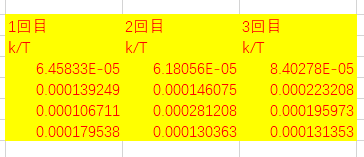
\includegraphics[width=\textwidth]{excel}
		\caption{Execl截图}
\end{figure}
\end{minipage}
\hfill
\begin{minipage}{0.45\textwidth}
	\centering
{\tiny	% Table generated by Excel2LaTeX from sheet 'Sheet1'


	\caption{表格示例}
	\begin{tabular}{rrr}
		\rowcolor[rgb]{ 1,  1,  0} \multicolumn{1}{l}{\textcolor[rgb]{ 1,  0,  0}{1回目}} & \multicolumn{1}{l}{\textcolor[rgb]{ 1,  0,  0}{2回目}} & \multicolumn{1}{l}{\textcolor[rgb]{ 1,  0,  0}{3回目}} \\
		\rowcolor[rgb]{ 1,  1,  0} \multicolumn{1}{l}{\textcolor[rgb]{ 1,  0,  0}{k/T}} & \multicolumn{1}{l}{\textcolor[rgb]{ 1,  0,  0}{k/T}} & \multicolumn{1}{l}{\textcolor[rgb]{ 1,  0,  0}{k/T}} \\
		\rowcolor[rgb]{ 1,  1,  0} \textcolor[rgb]{ 1,  0,  0}{6.45833E-05} & \textcolor[rgb]{ 1,  0,  0}{6.18056E-05} & \textcolor[rgb]{ 1,  0,  0}{8.40278E-05} \\
		\rowcolor[rgb]{ 1,  1,  0} \textcolor[rgb]{ 1,  0,  0}{0.000139249} & \textcolor[rgb]{ 1,  0,  0}{0.000146075} & \textcolor[rgb]{ 1,  0,  0}{0.000223208} \\
		\rowcolor[rgb]{ 1,  1,  0} \textcolor[rgb]{ 1,  0,  0}{0.000106711} & \textcolor[rgb]{ 1,  0,  0}{0.000281208} & \textcolor[rgb]{ 1,  0,  0}{0.000195973} \\
		\rowcolor[rgb]{ 1,  1,  0} \textcolor[rgb]{ 1,  0,  0}{0.000179538} & \textcolor[rgb]{ 1,  0,  0}{0.000130363} & \textcolor[rgb]{ 1,  0,  0}{0.000131353} \\
	\end{tabular}%


}
\end{minipage}
\end{table}

\par
在这里可以做个实验: 如果源代码中\verb|\hfill|的上下有空行, 则两者马上会错开到上下布局. 可见虽说\LaTeX 整体对缩进和空格不敏感\footnote{比Python强}, 但还是尽量标准一些写代码比较好.
\\\,\\
\verb|\hfill|上空行:
\begin{table}[h!]
	\centering
	\begin{minipage}{0.45\textwidth}
		\begin{figure}[H]
			\centering
			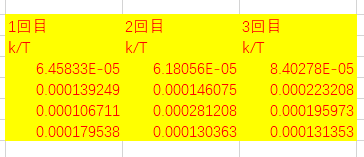
\includegraphics[width=\textwidth]{excel}
			\caption{Execl截图}
		\end{figure}
	\end{minipage}
	
	\hfill
	\begin{minipage}{0.45\textwidth}
		\centering
		{\tiny	% Table generated by Excel2LaTeX from sheet 'Sheet1'


	\caption{表格示例}
	\begin{tabular}{rrr}
		\rowcolor[rgb]{ 1,  1,  0} \multicolumn{1}{l}{\textcolor[rgb]{ 1,  0,  0}{1回目}} & \multicolumn{1}{l}{\textcolor[rgb]{ 1,  0,  0}{2回目}} & \multicolumn{1}{l}{\textcolor[rgb]{ 1,  0,  0}{3回目}} \\
		\rowcolor[rgb]{ 1,  1,  0} \multicolumn{1}{l}{\textcolor[rgb]{ 1,  0,  0}{k/T}} & \multicolumn{1}{l}{\textcolor[rgb]{ 1,  0,  0}{k/T}} & \multicolumn{1}{l}{\textcolor[rgb]{ 1,  0,  0}{k/T}} \\
		\rowcolor[rgb]{ 1,  1,  0} \textcolor[rgb]{ 1,  0,  0}{6.45833E-05} & \textcolor[rgb]{ 1,  0,  0}{6.18056E-05} & \textcolor[rgb]{ 1,  0,  0}{8.40278E-05} \\
		\rowcolor[rgb]{ 1,  1,  0} \textcolor[rgb]{ 1,  0,  0}{0.000139249} & \textcolor[rgb]{ 1,  0,  0}{0.000146075} & \textcolor[rgb]{ 1,  0,  0}{0.000223208} \\
		\rowcolor[rgb]{ 1,  1,  0} \textcolor[rgb]{ 1,  0,  0}{0.000106711} & \textcolor[rgb]{ 1,  0,  0}{0.000281208} & \textcolor[rgb]{ 1,  0,  0}{0.000195973} \\
		\rowcolor[rgb]{ 1,  1,  0} \textcolor[rgb]{ 1,  0,  0}{0.000179538} & \textcolor[rgb]{ 1,  0,  0}{0.000130363} & \textcolor[rgb]{ 1,  0,  0}{0.000131353} \\
	\end{tabular}%


}
	\end{minipage}
\end{table}

\clearpage

\verb|\hfill|下空行(新摆一页是因为前面放不下了):
\begin{table}[h!]
	\centering
	\begin{minipage}{0.45\textwidth}
		\begin{figure}[H]
			\centering
			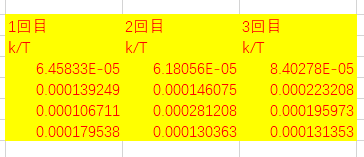
\includegraphics[width=\textwidth]{excel}
			\caption{Execl截图}
		\end{figure}
	\end{minipage}
	\hfill
	
	\begin{minipage}{0.45\textwidth}
		\centering
		{\tiny	% Table generated by Excel2LaTeX from sheet 'Sheet1'


	\caption{表格示例}
	\begin{tabular}{rrr}
		\rowcolor[rgb]{ 1,  1,  0} \multicolumn{1}{l}{\textcolor[rgb]{ 1,  0,  0}{1回目}} & \multicolumn{1}{l}{\textcolor[rgb]{ 1,  0,  0}{2回目}} & \multicolumn{1}{l}{\textcolor[rgb]{ 1,  0,  0}{3回目}} \\
		\rowcolor[rgb]{ 1,  1,  0} \multicolumn{1}{l}{\textcolor[rgb]{ 1,  0,  0}{k/T}} & \multicolumn{1}{l}{\textcolor[rgb]{ 1,  0,  0}{k/T}} & \multicolumn{1}{l}{\textcolor[rgb]{ 1,  0,  0}{k/T}} \\
		\rowcolor[rgb]{ 1,  1,  0} \textcolor[rgb]{ 1,  0,  0}{6.45833E-05} & \textcolor[rgb]{ 1,  0,  0}{6.18056E-05} & \textcolor[rgb]{ 1,  0,  0}{8.40278E-05} \\
		\rowcolor[rgb]{ 1,  1,  0} \textcolor[rgb]{ 1,  0,  0}{0.000139249} & \textcolor[rgb]{ 1,  0,  0}{0.000146075} & \textcolor[rgb]{ 1,  0,  0}{0.000223208} \\
		\rowcolor[rgb]{ 1,  1,  0} \textcolor[rgb]{ 1,  0,  0}{0.000106711} & \textcolor[rgb]{ 1,  0,  0}{0.000281208} & \textcolor[rgb]{ 1,  0,  0}{0.000195973} \\
		\rowcolor[rgb]{ 1,  1,  0} \textcolor[rgb]{ 1,  0,  0}{0.000179538} & \textcolor[rgb]{ 1,  0,  0}{0.000130363} & \textcolor[rgb]{ 1,  0,  0}{0.000131353} \\
	\end{tabular}%


}
	\end{minipage}
\end{table}
\,\\\,\\
\verb|\hfill|上下空行:
\begin{table}[h!]
	\centering
	\begin{minipage}{0.45\textwidth}
		\begin{figure}[H]
			\centering
			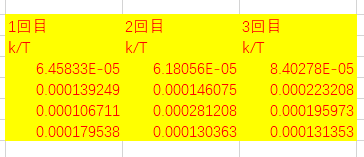
\includegraphics[width=\textwidth]{excel}
			\caption{Execl截图}
		\end{figure}
	\end{minipage}
	
	\hfill
	
	\begin{minipage}{0.45\textwidth}
		\centering
		{\tiny	% Table generated by Excel2LaTeX from sheet 'Sheet1'


	\caption{表格示例}
	\begin{tabular}{rrr}
		\rowcolor[rgb]{ 1,  1,  0} \multicolumn{1}{l}{\textcolor[rgb]{ 1,  0,  0}{1回目}} & \multicolumn{1}{l}{\textcolor[rgb]{ 1,  0,  0}{2回目}} & \multicolumn{1}{l}{\textcolor[rgb]{ 1,  0,  0}{3回目}} \\
		\rowcolor[rgb]{ 1,  1,  0} \multicolumn{1}{l}{\textcolor[rgb]{ 1,  0,  0}{k/T}} & \multicolumn{1}{l}{\textcolor[rgb]{ 1,  0,  0}{k/T}} & \multicolumn{1}{l}{\textcolor[rgb]{ 1,  0,  0}{k/T}} \\
		\rowcolor[rgb]{ 1,  1,  0} \textcolor[rgb]{ 1,  0,  0}{6.45833E-05} & \textcolor[rgb]{ 1,  0,  0}{6.18056E-05} & \textcolor[rgb]{ 1,  0,  0}{8.40278E-05} \\
		\rowcolor[rgb]{ 1,  1,  0} \textcolor[rgb]{ 1,  0,  0}{0.000139249} & \textcolor[rgb]{ 1,  0,  0}{0.000146075} & \textcolor[rgb]{ 1,  0,  0}{0.000223208} \\
		\rowcolor[rgb]{ 1,  1,  0} \textcolor[rgb]{ 1,  0,  0}{0.000106711} & \textcolor[rgb]{ 1,  0,  0}{0.000281208} & \textcolor[rgb]{ 1,  0,  0}{0.000195973} \\
		\rowcolor[rgb]{ 1,  1,  0} \textcolor[rgb]{ 1,  0,  0}{0.000179538} & \textcolor[rgb]{ 1,  0,  0}{0.000130363} & \textcolor[rgb]{ 1,  0,  0}{0.000131353} \\
	\end{tabular}%


}
	\end{minipage}
\end{table}

\end{appendices}







\end{document}
